\documentclass[11pt,a4paper]{article}
\usepackage[margin=23mm]{geometry}
\usepackage[T1]{fontenc}
\usepackage{lmodern}
\usepackage{hyperref}
\emergencystretch=2em
\usepackage{tikz}
\usetikzlibrary{positioning,arrows.meta}
\title{Core canonical identity as one object: \texttt{canon.hash()}}
\date{Created-at: 2026-09-29 18:49 +02:00\quad ETA: about 2.5\,h (Canon and its identity 0.5\,h; 94 Core call sites 0.5\,h; tests and gates 0.5\,h; Nagare repin, migration and A/B 1\,h)}
\begin{document}
\maketitle

\paragraph{Request.} User, 2026-09-29: fetch the newest version of core. The hash should be computed'';
create new branch on feature. We need cannon.hash() or more structural and object oriented''.
Core and its remote were fetched at 18:47; \texttt{origin/main} is \texttt{9a236ac}, Nagare's pin
\texttt{fb94550} plus two documentation commits. Branch \texttt{feat/canonical-identity} from it,
upstream unset.

\paragraph{Evidence.}
\begin{itemize}
\item \texttt{ModuleStore::compile} computes the structural V1 hash (\texttt{canon\_hash}) and the
  deprecated declaration Merkle table; it computes no semantic identity. Its own comment names
  \texttt{semantic\_model\_digest\_v2} as the sound identity''.
\item V1 is blind to values: with Core's CLI, \texttt{vertex\_index 1}$\to$\texttt{7} and
  \texttt{slot "s"}$\to$\texttt{"t"} keep the hash; one arc sign changes it.
\item Identity is a flat family of free functions over \texttt{(ir, interner)}:
  \texttt{canonical\_program\_hash}, \texttt{program\_structure\_hash\_v1},
  \texttt{semantic\_model\_digest\_v2}, \texttt{semantic\_declaration\_hashes}; each derives the
  canonical paths again (\texttt{CanonicalPaths}, \texttt{build\_path\_index}).
\item Nagare computed the source digest itself until \texttt{faa22b8}; the user placed it in Core.
\end{itemize}

\paragraph{Design.}
\begin{itemize}
\item \texttt{Canon<'ir>}: the canonical view of one IR -- the IR, its interner, its path index
  derived once. Methods \texttt{hash()} (semantic V2 digest), \texttt{structure(cfg)} (V1),
  \texttt{declaration\_hashes()}, \texttt{paths()}, \texttt{validate(idx)} (the lowering-boundary
  check). It replaces the four free functions and the crate-private \texttt{CanonicalPaths}.
\item \texttt{CanonicalIdentity}: the value a compile keeps -- \texttt{hash()} and
  \texttt{structure()} -- computed once in \texttt{ModuleStore::compile} through one \texttt{Canon}.
  \texttt{CompiledProgram::canon} replaces \texttt{canon\_hash}: \texttt{program.canon.hash()}.
\item Unchanged: every hash byte (known-answer vectors), the CBOR wire field \texttt{canon\_hash}
  (data, written from \texttt{Canon::structure}), the deprecated Merkle pass (classified ambiguous
  by Core, untouched), \texttt{build\_path\_index}.
\end{itemize}

\paragraph{CORE.YAML.} \texttt{hymeko\_core} is \texttt{lockdown: full}. This change needs
\texttt{APPROVED-CORE-EDIT: canonical-identity}; its entry is added to \texttt{approved\_edits} in the
same change. Scope: \path{hymeko_core/src/ir/{canonical_hash,semantic_digest}.rs},
\path{module_store/module_store.rs}, \path{writers/cbor_writer.rs} and its \texttt{validate.rs},
\path{util/pretty_print.rs}, \path{ir/{coherence,time}.rs}, the tests, benches and example that call
the replaced functions (94 sites). Constraints: no hash value changes; no wire change; no dependency.

\paragraph{Consumers.} Nagare migrates in this work after a local-path build (no push): the source
identity is \texttt{program.canon}, the model digest \texttt{Canon::new(ir, it).hash()}. Listed, not
edited, migrate at their next repin: \path{graph/hymeko_graph/tests/ir_ops_bench.rs},
\path{transformation/hymeko_emitter/tests/fault_mutants.rs}, \path{network/src/optimize.rs},
\path{application/hymeko_daemon/src/worker.rs}.

\paragraph{Tests.} Existing known-answer and coverage suites (\path{frozen_hash.rs},
\path{semantic_digest.rs}, \path{identity.rs}, \path{hash_coverage.rs}) run unchanged through the
methods: bit identity. New: a compiled program's \texttt{canon} equals \texttt{Canon} of its IR;
\texttt{hash()} separates the two value changes \texttt{structure()} cannot. Core gate, then Nagare's
\texttt{scripts/check.sh} and its eight regression records bit for bit.

\paragraph{Performance budget.} Core's compile gains one semantic digest and loses one path
derivation. Nagare at CogInfoCom Alpha (seed 0, 20 passes, runner settings): compile at most
13.0\,s (the \texttt{c1a155e} level, which computed this digest in Nagare), peak RSS 2243\,MiB.

\paragraph{Rollback.} The branch is unpushed; Nagare keeps its pin until the repin commit.

\paragraph{Risks.} Every Core compile now pays for the semantic digest, consumers that never read
it included. The four listed consumers break at their next repin until migrated. A method whose
bytes differ from the free function it replaces fails the known-answer suites.

\begin{center}
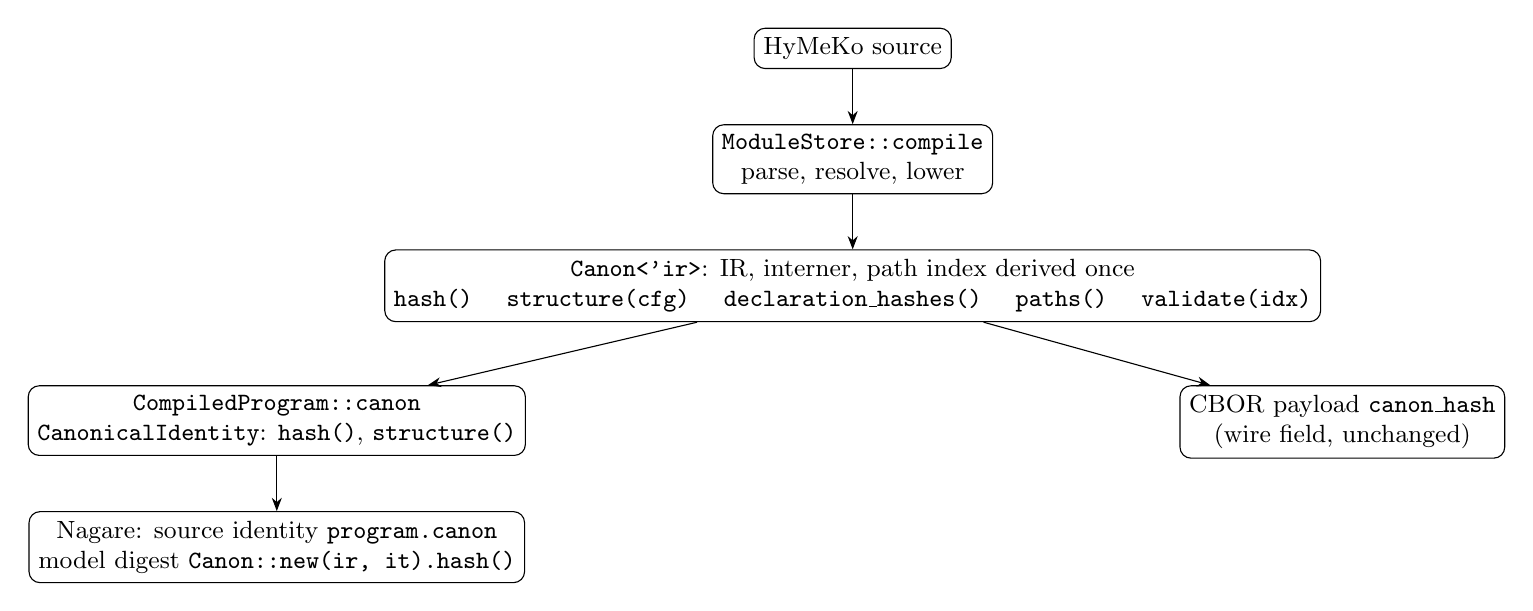
\begin{tikzpicture}[node distance=7mm,every node/.style={draw,rounded corners,align=center,font=\small},>={Stealth}]
\node (src) {HyMeKo source};
\node (store) [below=of src] {\texttt{ModuleStore::compile}\\parse, resolve, lower};
\node (canon) [below=of store] {\texttt{Canon<'ir>}: IR, interner, path index derived once\\\texttt{hash()} \quad \texttt{structure(cfg)} \quad \texttt{declaration\_hashes()} \quad \texttt{paths()} \quad \texttt{validate(idx)}};
\node (id) [below left=8mm and -18mm of canon] {\texttt{CompiledProgram::canon}\\\texttt{CanonicalIdentity}: \texttt{hash()}, \texttt{structure()}};
\node (wire) [below right=8mm and -18mm of canon] {CBOR payload \texttt{canon\_hash}\\(wire field, unchanged)};
\node (nagare) [below=of id] {Nagare: source identity \texttt{program.canon}\\model digest \texttt{Canon::new(ir, it).hash()}};
\draw[->] (src)--(store); \draw[->] (store)--(canon); \draw[->] (canon)--(id); \draw[->] (canon)--(wire); \draw[->] (id)--(nagare);
\end{tikzpicture}
\end{center}

\end{document}
